\section{System Architecture} % Maybe change to "simulation architecture"

\begin{comment}
\begin{figure}[t]
\centering
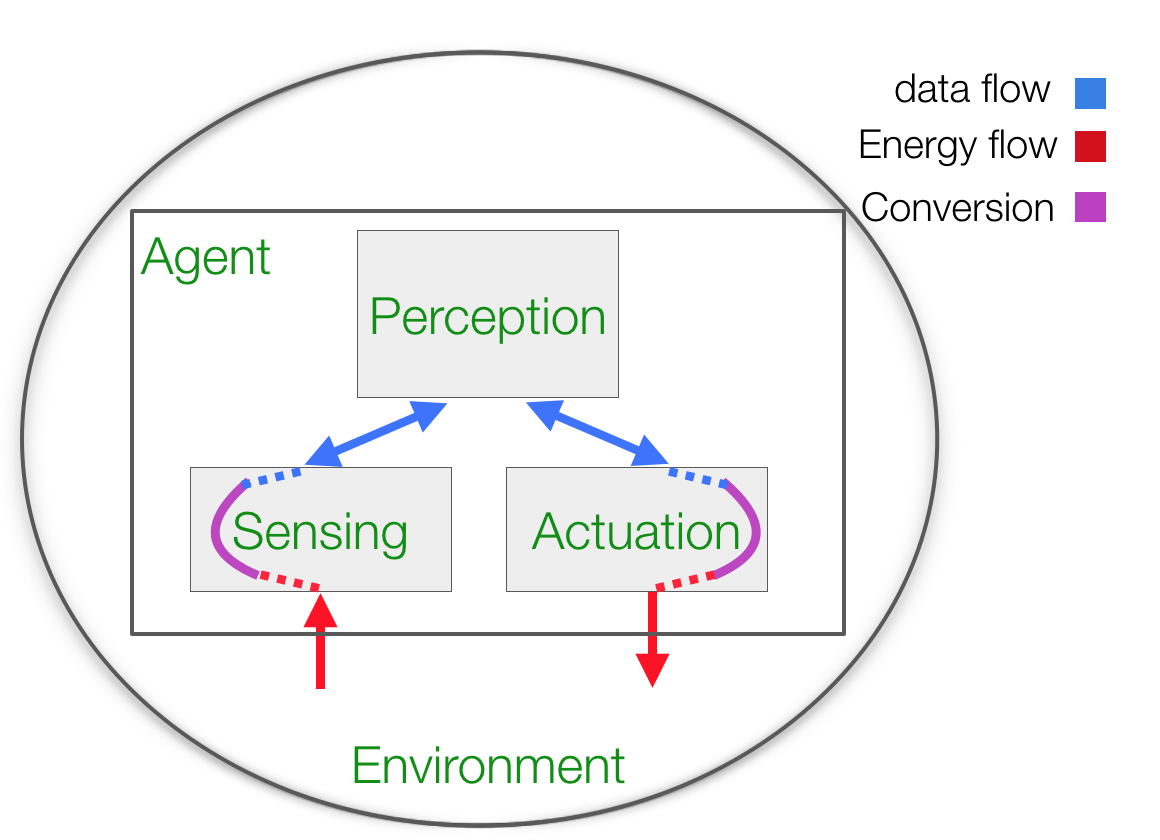
\includegraphics[width=6cm, height=4cm ,keepaspectratio]{figs/robot_arch.png}
\caption{System architecture of a typical robotic agent.}
\end{figure}
\end{comment}
%In this section, we provide an architectural overview of typical drone platforms in order to provide the background necessary to understand their architectural constraints, and the requirements for a simulator that can provide insights into those constraints.

% \textcolor{red}{Like any other robotic systems, drones have 3 subsystems: ....}
%\subsection{Accuracy Impact:}
\begin{figure}[t!]
\centering
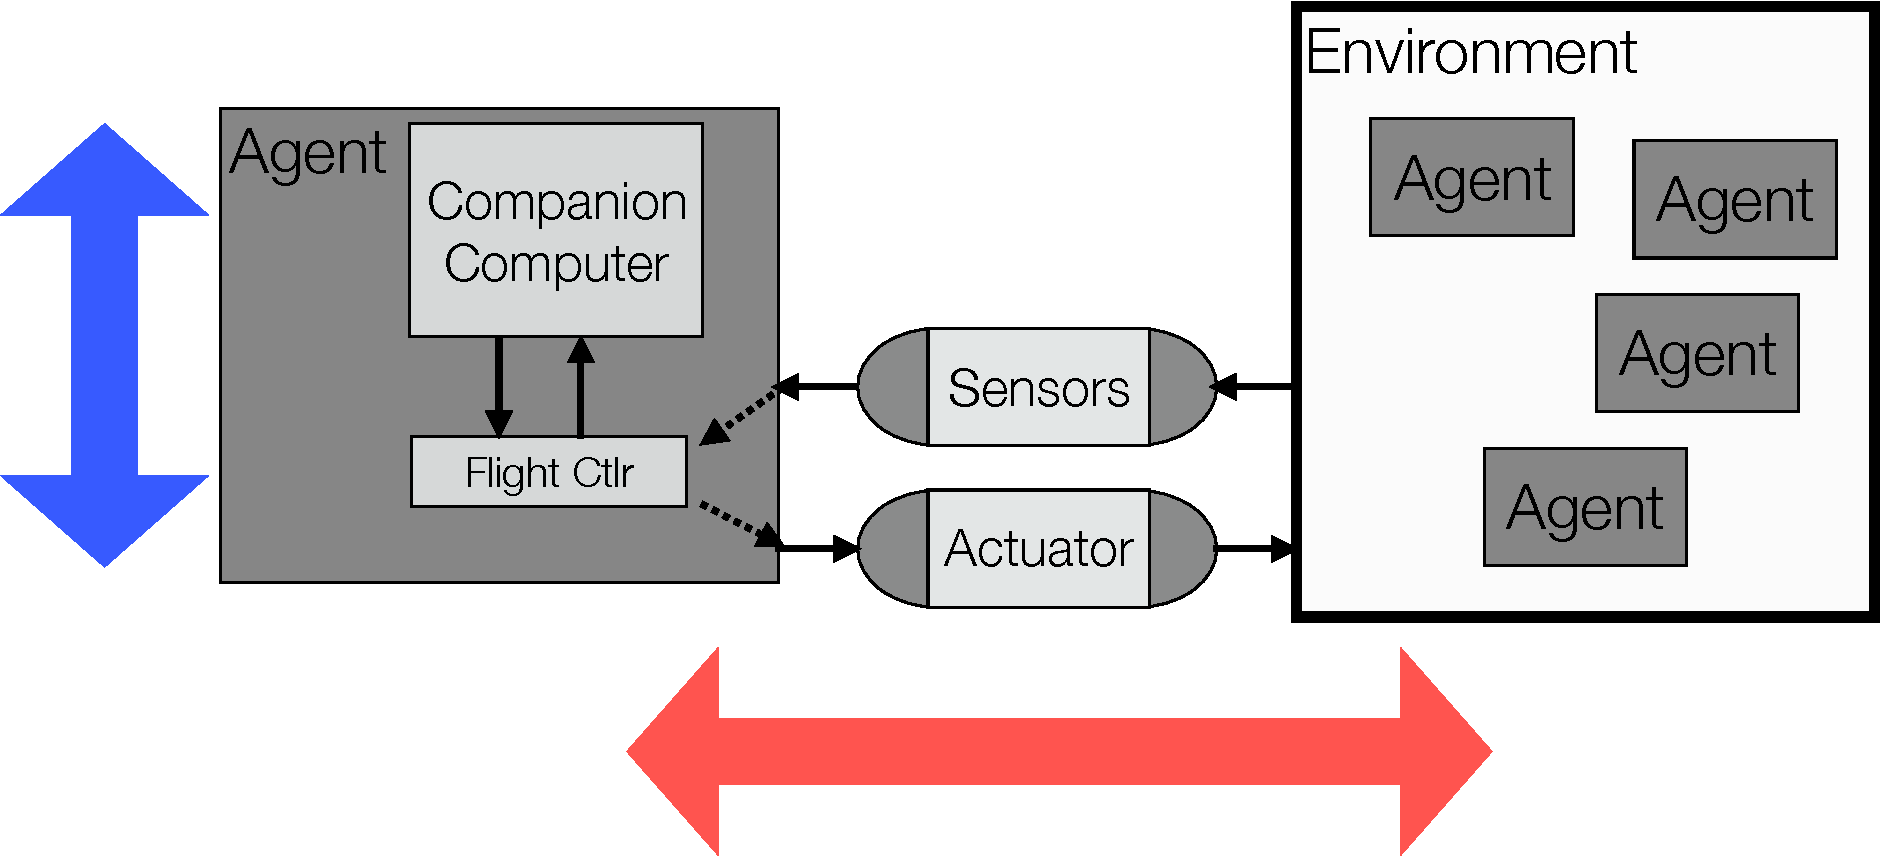
\includegraphics[width=0.9\columnwidth]{figs/agent_env.pdf}
\vspace{1.0ex}
\caption{Agent-environment model.}
\vspace{-3ex}
\label{fig:1}
\end{figure}
Given the aforementioned constrains, these agents demand architects attention. In this section, we provide the architectural overview of such agents as the first step toward a design around such constrains.  

Like other robotic agents, such systems operate by sampling the environment state, interpreting and reacting to it using three main subsystems, namely, a sensory subsystem, a perception subsystem, and an actuation subsystem. Fig.~\ref{} shows these subsystems and their corresponding data and energy flow. More concretely, Fig.~\ref{} shows the details of each subsystem \textcolor{red}{(have various sensors and actuator names on the figure.)}
\begin{comment}
\begin{figure}
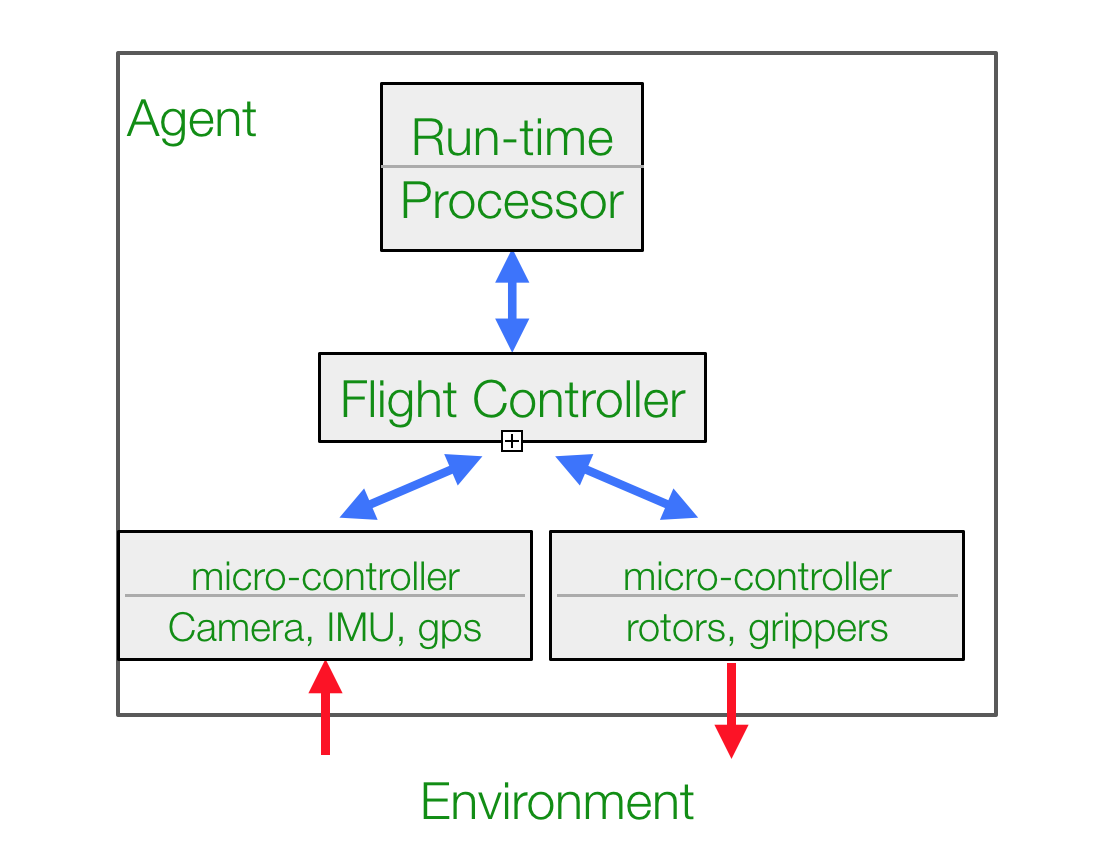
\includegraphics[width=6cm, height=4cm ,keepaspectratio]{figs/drone_arch.png}
\caption{Detailed system architecture of an aerial robotic agent.}
\end{figure}
\end{comment}
\begin{comment}
Sensor subsystem: is usually comprised of a versatile set of sensors such as cameras, IMU (inertial measurement units), IR, lidar, etc depending on size, energy budget and other constraints.
Perception subsystem: This system is responsible for processing the sampled data. typical off-the-shelf UAVs, such as the 3DR Solo, are equipped with at least two on-board processors: a ``companion computer'' that handles workloads, and a ``flight controller'' responsible for high to low (and vice versa) conversion of sensing and actuation subcommands (e.g. conversion of hover (high level) command to specific rotor speed (low level)).
Actuation subsystem: this system is responsible for reacting and modifying the world around the agent. It ranges anywhere from rather simple rotors to robotic arms capable of grasping and lifting objects. 
}


\begin{figure}[h]
\centering
\includegraphics[width=\linewidth]{figs/drone-architecture}
\caption{Architectural overview of a typical drone platform. \textcolor{red}{Iterate over this figure; it should be improved.}}
\label{fig:dronearch}
\end{figure}
\end{comment}

\textbf{Sensory Subsystem} To enable intelligent flight, drones must be equipped with a rich set of sensors that are capable of gathering visual, depth, position, and orientation data. For example, to detect possible intruders and separate them from authorized visitors, an autonomous security drone will require image data from cameras. To detect the positions of obstacles, a drone would also require depth information from stereo or RGBD cameras. Number and type of sensors is highly dependent on the workload requirement such as, and various system constraints such as perception subsystem capability to process them. 

\textbf{Perception Subsystem} To enable intelligent flight, drones must also come equipped with on-board companion computers that are capable of performing high-level cognitive \textcolor{red}{(this probably isn't the right word here)} tasks, such as object classification and obstacle avoidance. Such processors must satisfy various constraints such as drone's thermal and energy limit,form factor, etc. Therefore, many off-the-shelf drone platforms such as the Solo come equipped with small, low-power processors such as the ARM Cortex-M A9 that struggle to provide real-time cognitive capability for compute-heavy tasks such as visual classification. For higher performance, UAV designers can turn to other state-of-the-art embedded systems such as the NVIDIA TX2, although these systems incur higher power penalties. In addition to the companion computers, typically, drone platforms come with a ``flight controller'' responsible for high to low (and vice versa) conversion of sensing and actuation subcommands (e.g. conversion of hover (high level) command to specific rotor speed (low level).

\textbf{Actuation Subsystem} This system is responsible for reacting and modifying the world around the agent. It ranges anywhere from rather simple rotors to robotic arms capable of grasping and lifting objects.
Similar to sensors, their type and number is highly a function of the workload and processing power on board. 
